\documentclass[draftclsnofoot, onecolumn, compsoc, 10pt]{IEEEtran}
\usepackage{lscape}
\usepackage{rotating}
\usepackage{titling}
\usepackage[margin=0.75in]{geometry}
\usepackage{graphicx}
\usepackage{placeins}
\usepackage{caption}
\usepackage{float}
\usepackage{url}
\usepackage{natbib}
\usepackage{setspace}
\geometry{textheight=9.5in, textwidth=7in}
\graphicspath{ {images/} }
\linespread{1.0}
\parindent=0.0in
\parskip=0.2in

\title{\huge Software Design Document}
\author{Oregon State University\\CS 461\\2017-2018\\\\Prepared By:\\ Kyle Prouty\\Hayden Anderson\\}

\def \CapstoneTeamName{		Rodents Of Unusual Size}
\def \CapstoneTeamNumber{		46}
\def \GroupMemberOne{			Hayden Anderson}
\def \GroupMemberTwo{			Kyle Prouty}
\def \CapstoneProjectName{		Project ROUS}
\def \CapstoneSponsorCompany{	HP, Inc}
\def \CapstoneSponsorPerson{	Lonnie Mandigo}

\def \DocType{ Design Document }
			
\newcommand{\NameSigPair}[1]{\par
\makebox[2.75in][r]{#1} \hfil 	\makebox[3.25in]{\makebox[2.25in]{\hrulefill} \hfill		\makebox[.75in]{\hrulefill}}
\par\vspace{-12pt} \textit{\tiny\noindent
\makebox[2.75in]{} \hfil		\makebox[3.25in]{\makebox[2.25in][r]{Signature} \hfill	\makebox[.75in][r]{Date}}}}

\begin{document}
\begin{titlepage}
    \pagenumbering{gobble}
    \begin{singlespace}
        \hfill  
        \par\vspace{.2in}
        \centering
        \scshape{
            \huge CS Capstone \DocType \par
            {\large\today}\par
            \vspace{.5in}
            \textbf{\Huge\CapstoneProjectName}\par
            \vfill
            {\large Prepared for}\par
            \Huge \CapstoneSponsorCompany\par
            \vspace{5pt}
            {\Large\NameSigPair{\CapstoneSponsorPerson}\par}
            {\large Prepared by }\par
            Group\CapstoneTeamNumber\par
            \CapstoneTeamName\par 
            \vspace{5pt}
            {\Large
                \NameSigPair{\GroupMemberOne}\par
                \NameSigPair{\GroupMemberTwo}\par
            }
            \vspace{20pt}
        }
        \begin{abstract}
        \noindent 
        This document will examine the design of our software framework. It will look at the overall framework design, then go into a detailed look at the software, hardware, and graphical user interface that will make up our framework. Overall, this document will layout the specifics of how our framework will be designed so that it meets all the requirements.
%         In this document, the ROUS project in its entirety is explained. The timeline of when each part to be implemented as well as how each piece of the ROUS system will be accomplished. This document will also go over how the project will be tested.
        \end{abstract}     
    \end{singlespace}
\end{titlepage}
\newpage
\pagenumbering{arabic}
\clearpage 
\tableofcontents
\pagebreak




\section{Introduction}
\subsection{Overview}
The framework being developed will create a network of nodes that will communicate by broadcasting simple messages to each other. Nodes will use network protocols to pass these messages in order to self organize on an objective. Users will be able to input print job objectives into our framework and view the results from a graphical user interface.

Sections below take an in depth look at the design of the framework. These sections begin by taking a high level look at the overall design and then go into the specifics of how each piece of the framework is working together to accomplish an objective.

\subsection{Purpose}
Overall the rationale for the entire framework is to have a collection of loosely coupled nodes that can self organize to accomplish a print job. This framework will be robust in the face of any nodes that become untrusted. Nodes in this framework will communicate with each other using simple messages over wireless network protocols. 
% Our framework's purpose is to enable a collection of loosely coupled nodes to be robust in the face of any mistrusted node. The framework will give these nodes the ability to self organize on an objective. It will allow the input of a structured print job objective and will be able to self organize to accomplish that objective. This robust framework will be able to accomplish objectives without each node having rigid logical configurations.
% The purpose of this document is to give details on the design of the ROUS framework. By the end of this document, the reader will understand the concepts needed to create an IoT framework that will perform robustly and collaborate.

\subsection{Scope}
The scope of this project will includes using a combination of software and hardware to develop a framework for passing messages between a collection of loosely coupled nodes. Software will contain core framework functionality along with the graphical user interface. 

\subsection{Audience}
The intended audience is our client and mentor, Lonnie Mandigo. It also includes the professors of our senior design capstone class, Kirsten Winters and Kevin McGrath.

\subsection{Glossary}
\subsubsection{Definitions, Acronyms, Abbreviations}
\bgroup
  \def\arraystretch{1.5}
  \resizebox{\textwidth}{!}{
  \begin{tabular}{| p{11.0cm} | p{11.0cm} |}
  \hline	
  \bf{Term} & \bf{Definition}\\
  \hline
  Node & The physical device that makes a piece of our network and provides functionality that can be applied to a variety of tasks\\
  \hline
  GUI & Graphical user Interface \\
  \hline
  TCP & Transmission Control Protocol: IP protocol that allows for reliable connection oriented communication between nodes \\
  \hline
  UDP & User Datagram Protocol: IP protocol that allows for connectionless communication between nodes  \\
  \hline
  Broadcast  & A networking signal to everyone on a network \\
  \hline
  Multicast & A networking signal to many destinations on the network \\
  \hline
  Raspberry Pi & A physical small form-factor platform used to hold our framework \\
  \hline
  Resin.io & Framework to help maintain and deploy code to Internet of things devices \\
  \hline
  ReactJS & A set of libraries for the JavaScript programming language designed for creating single page applications\\
  \hline
  \end{tabular}
  }
\egroup
\bibliographystyle{plain}
\bibliography{bibtex.bib}
\nocite{*}
\newpage



\section{Overall Framework Design}
\subsection{Architecture}
The ROUS framework being implemented will be organized into three parts: software, hardware, and a graphical user interface. These separate pieces will work together to make up the overall framework. This system will have the functionality to be given a print job objective, organize on that objective, and then accomplish that print job objective.

In this framework all communication happens by broadcasting simple messages. A user interface will provide users, observers, and administrators the ability to interact with the framework. The framework will contain a network of nodes that communicate by broadcasting simple messages. 
\begin{figure}[H]
\centering
	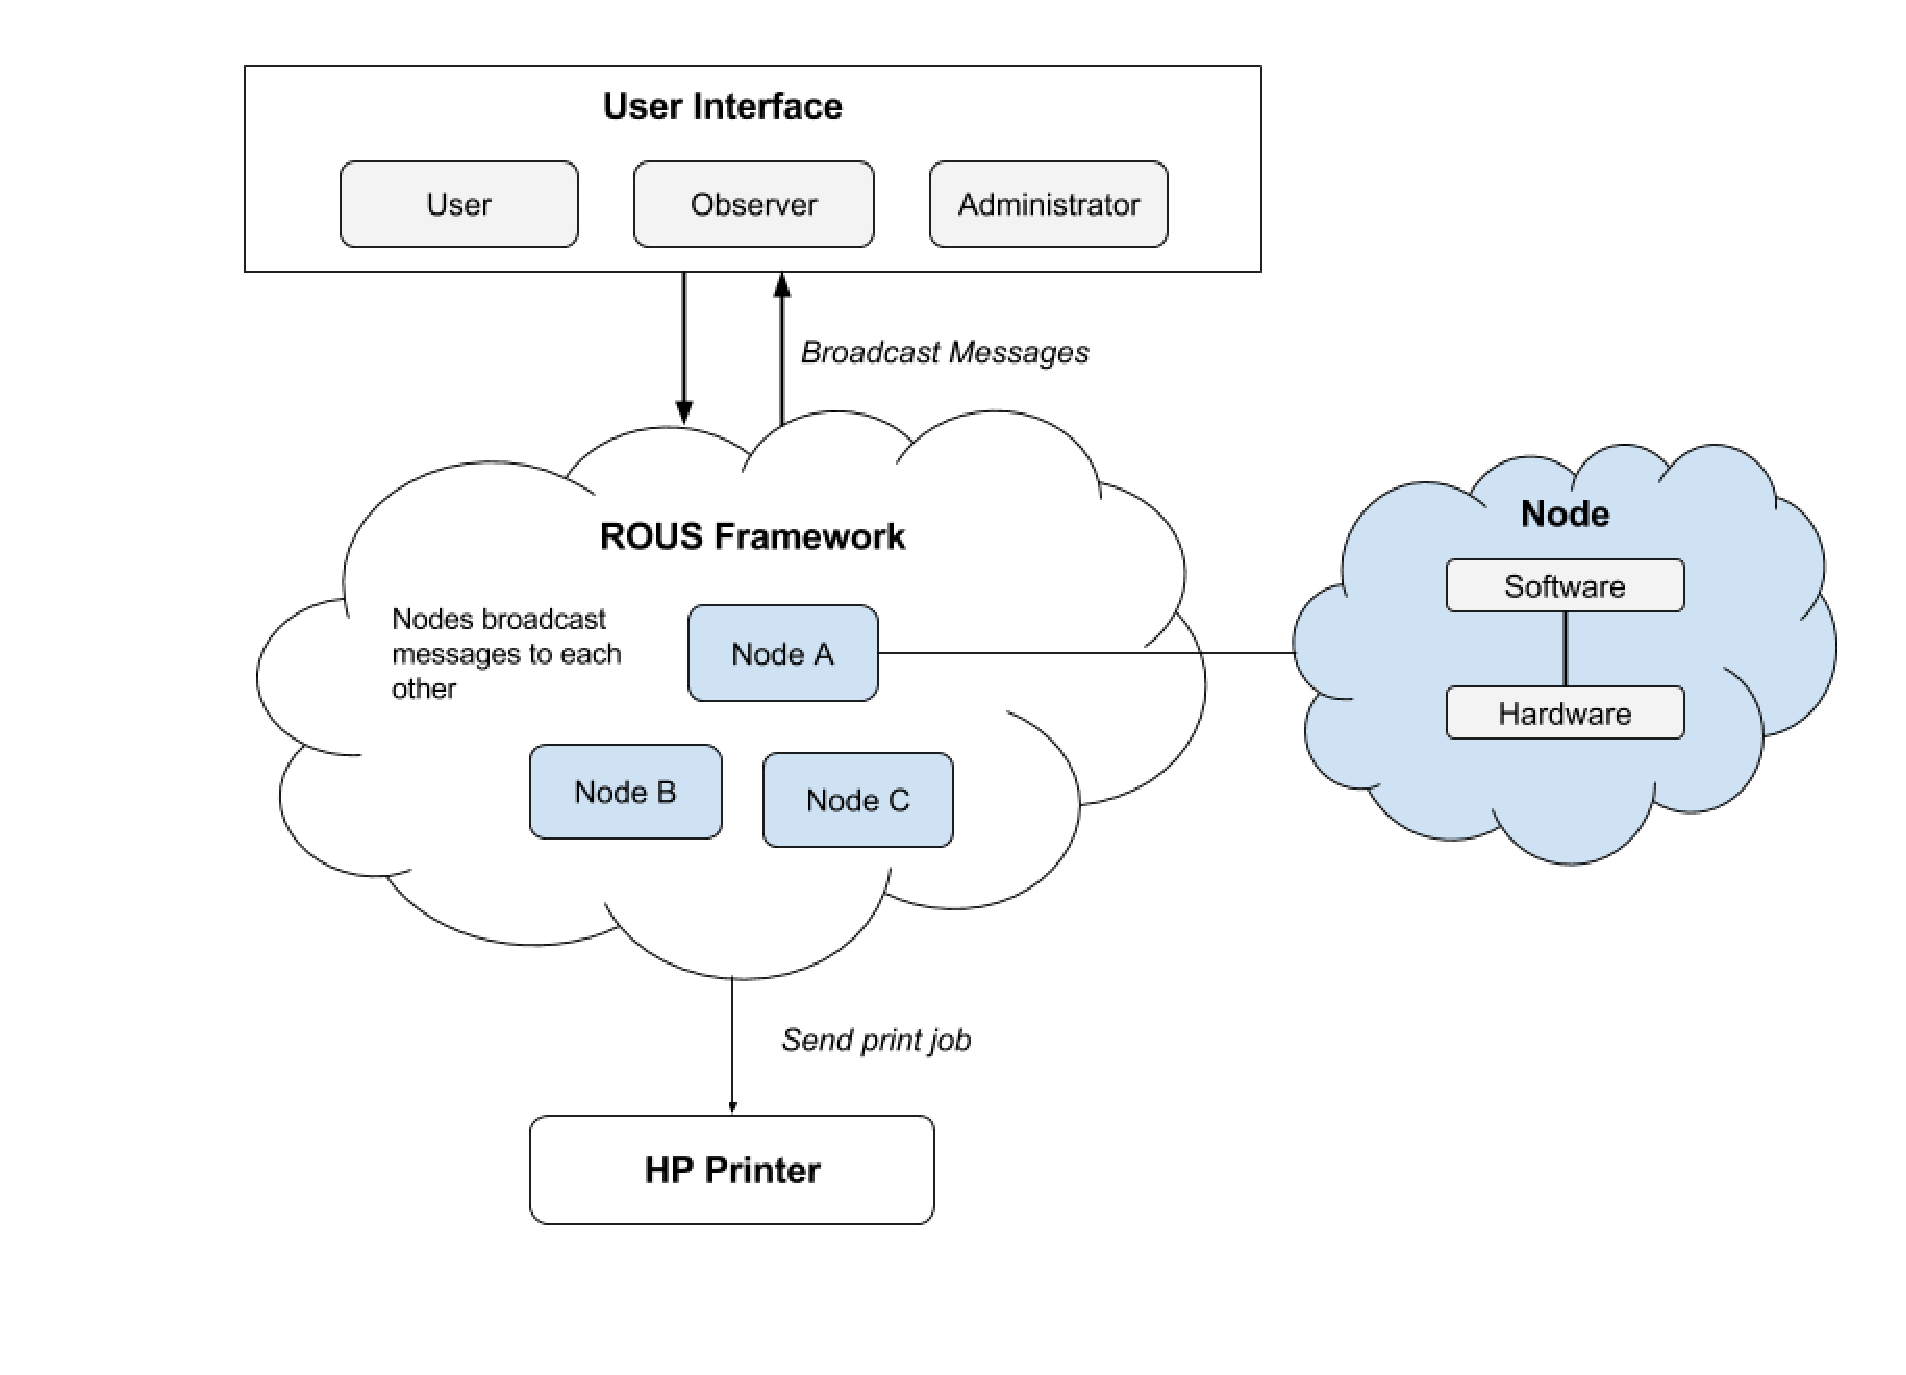
\includegraphics[scale=.55]{context}
	\captionsetup{justification=centering}
    \caption{This is a basic context view of the overall architecture of the ROUS framework}
\end{figure}

% \subsection{Rationale}
% Overall the rationale for the entire framework is to have a collection of loosely coupled nodes that can self organize to accomplish a print job. This framework will be robust in the face of any nodes that become untrusted. Nodes in this framework will communicate with each other using a complex language of messages over wireless Internet protocols. 

\subsection{Actors}
\subsubsection{User}
Users only care about the ability to input a print job objective and have that printed output appear on their printers. They will not care about how the framework accomplishes these goals. These end users will not have the ability to affect the framework in any way other than inputting a print job and viewing the results.

\subsubsection{Administrator}
Administrators perceive the framework in a different light than a user. These end users have the ability to see a more detailed look at the configuration and status of the framework. They also have the capabilities of seeing all services that each node offers and to disable those services. By disabling services these administrators are the end users who introduce sources of mistrust into the framework.

\subsubsection{Observer}
An observer is someone that wants to see how the framework works. These end users will be able to see configuration setting and the state of the system. They will also be able to see all the nodes on the network and their services, and be able to see the state of those services.

\section{Software}
\subsection{Overview}
Our software framework will be built on top of a Linux kernel using hardware that will allow our framework to have access to wireless network protocols. Overall, this software framework will enable nodes to self organize on objectives without the need for any rigid logical configurations. The subsections below will take a detailed look at how nodes will communicate, what capabilities each node will have, and give an examination of what a source of mistrust means to the system.

\subsection{Node Communication}
\subsubsection{Network Communication}
Basic node communication will happen over a partial ad hoc wireless network. A partial ad hoc network will be used because nodes will only be directly connected to each other when accessing print job objectives from other nodes. Most communication will happen via broadcasting a simple messages that each node will understand.

To accomplish network communication the framework will leverage two different transport network protocols, TCP and UDP. The protocol TCP will be used to transfer objective print job data from node to node. This protocol will be used because it will allow the framework to guarantee that packets will be delivered successfully and without error. 

In order to allow nodes to broadcast to multiple nodes at once, the framework will need to be able to use multi-cast. TCP does not allow multi-cast so the UDP transport protocol will be used for this feature. The framework will leverage the UDP protocol so that each node can broadcast a message to all nodes in the network. 

\subsubsection{Broadcasting}
Broadcasting will be the most important feature in how nodes communicate with other nodes. Since the goal is to design a framework that is loosely coupled, nodes will almost never be directly connected to each other in a tightly coupled way. To solve this issue, nodes will only communicate by broadcasting simple messages to each other.

Each node will have the ability to broadcast messages to any node in the network. These nodes will also be able to listen for messages that were broadcast. They will send response messages. This is how basic communication works, a simple message that contains a print job objective is broadcast to all nodes. If a node can perform that objective it will response with a bid. The original node who sent the original message will then send the objective to the node that won the bid. 

The figure below illustrates how this sequence of message passing works.

% In the basic sense this communication will work as such, node one broadcasts message A, all other nodes listen to message A, assume node two meets the requirements message A calls for, then node two will respond via broadcast with message B. Node one listens and sees that node two responded with message B which then tells node one to either complete an objective or respond again with a new message C. This process will repeat until the print job objective has been successfully completed.
\begin{figure}[H]
\centering
	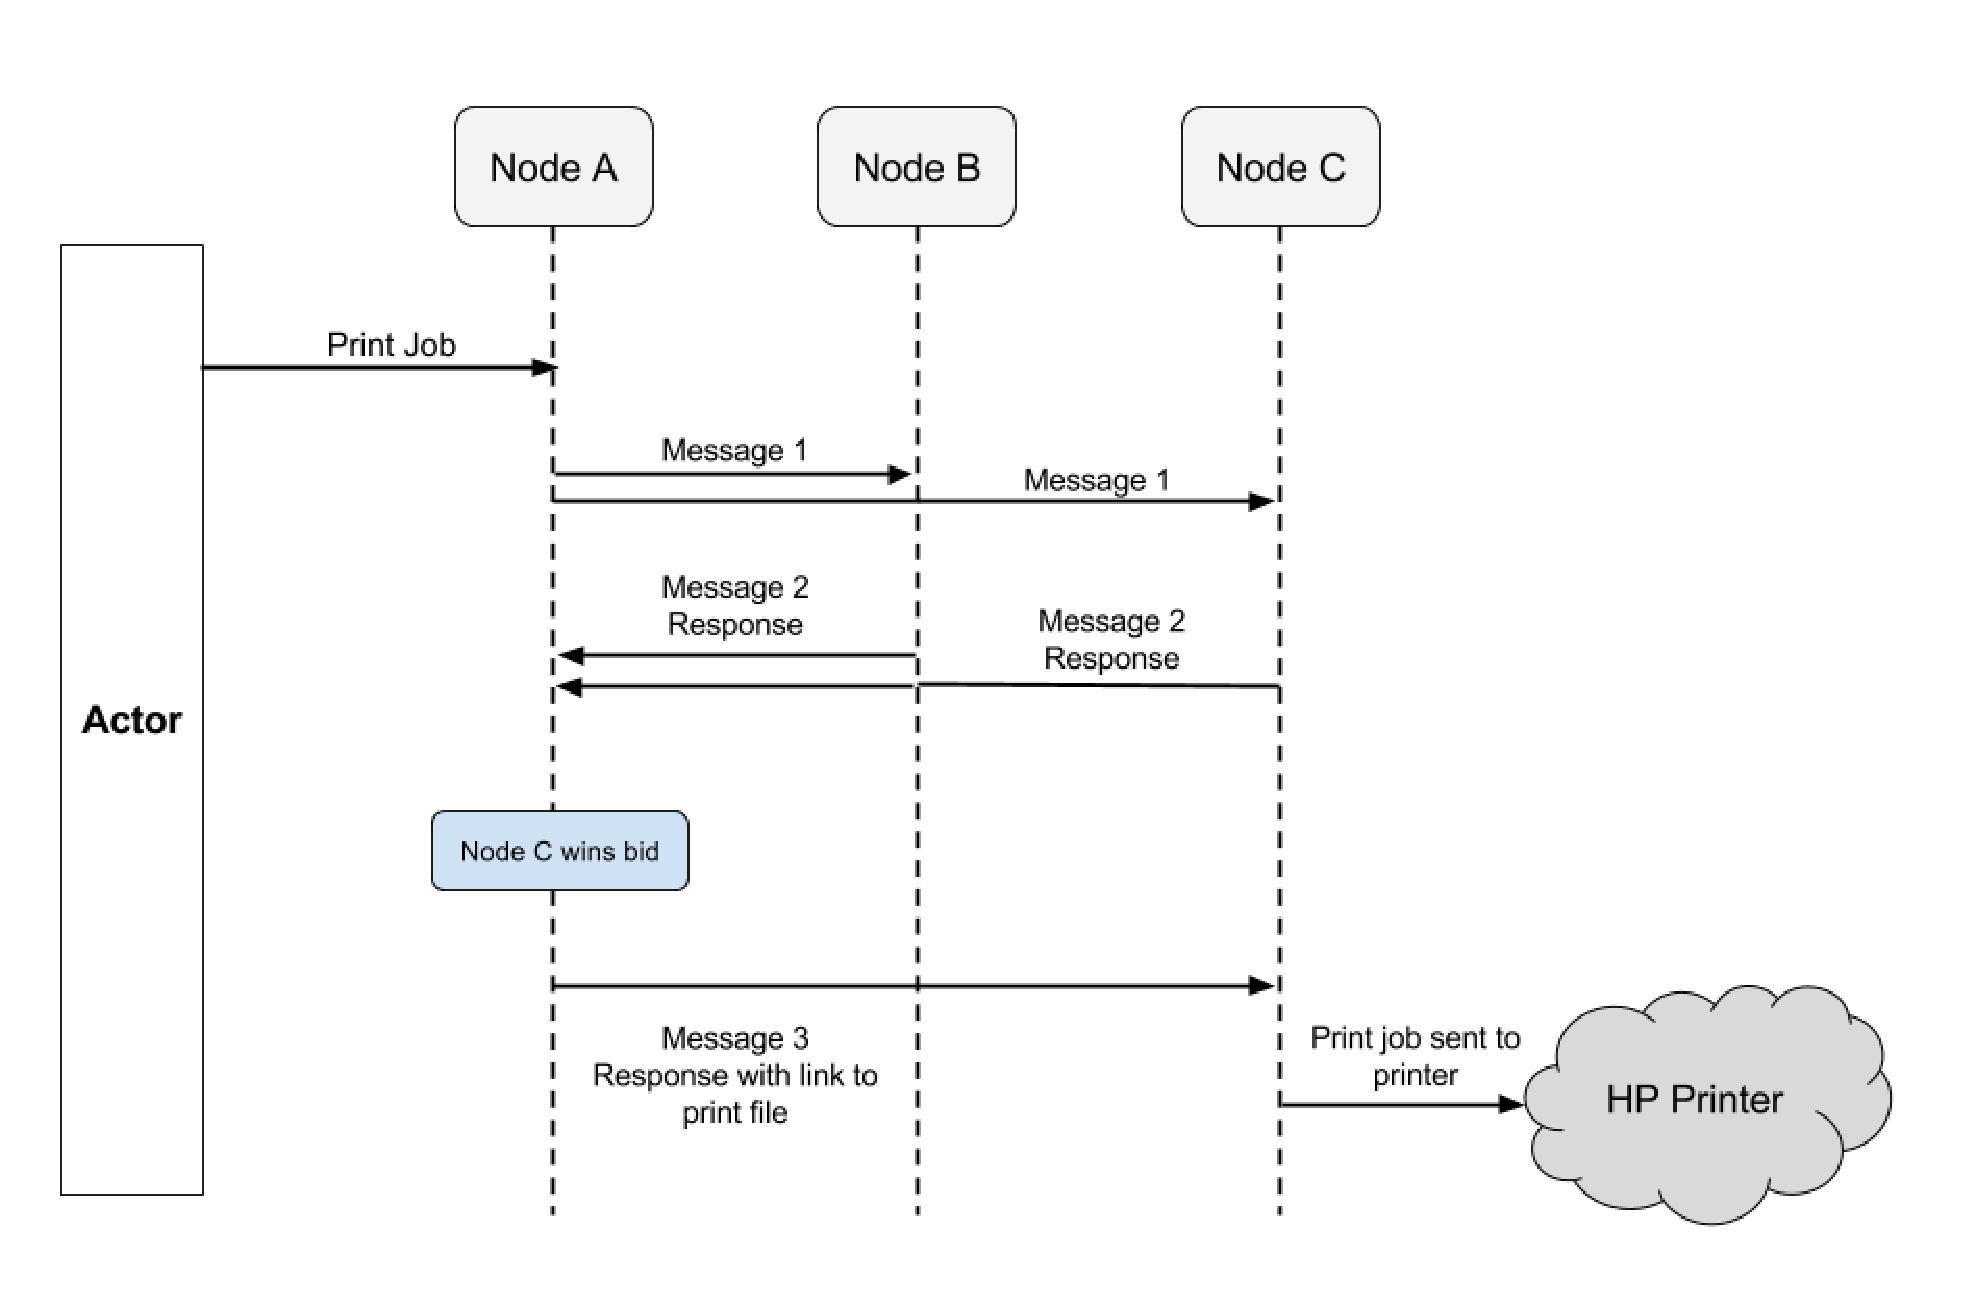
\includegraphics[scale=0.5]{sequence}
	\captionsetup{justification=centering}
    \caption{This illustrates a simple interaction between three nodes with the objective of printing a print job}
\end{figure}

\subsubsection{Messages}
Simple message passing is the heart of how nodes will communicate to accomplish objectives. A simple message will contain a keyword, followed by the parameters that go with that keyword. Nodes will first look at a messages keyword to determine if they need to look for any parameters. 

As an example, a message will be sent with the keyword \textit{print} followed by the parameters \textit{color}. Any node that can first accept a \textit{print} keyword and then accept a \textit{color} parameter will response. All nodes will communicate using this simple message  \textit{keyword:parameter} format. 
% A complex language will be the heart of how nodes communicate with other nodes. When a node broadcasts messages, each message will be part of this complex language. Each node will know how to interpret this complex language in order for it to self organize and complete print job objectives.

% Overall, this language will be complex enough that each node will have no ambiguity about what is being asked, but it will also be simple enough that no rigid logical configurations exist on any nodes.


\subsection{Node Capabilities}
\subsubsection{Services}
Every node in the framework will have a print job service. This print job service will give every node the ability to print an objective that has been inputted into the system. A service can be disabled by an administrator.

\subsubsection{Bidding}
An important capability that each node will have is the ability to bid on services that it can complete. When another node broadcasts a message and more then one node responds, bidding then occurs. Each node will bid for the ability to be the node that is tasked with accomplishing the current print job objective. The node that one the bid will not be able to bid on new objective until it has completed the objective that it one the bid for. Nodes that lost the bid will then be available to bid on any new objective that is input in the framework.

% Each node has specific services it can complete. Some services may have subsections of the service; e.g. A printer service that can only print black and white. When a node receives the objective, it broadcasts asking for a bid number from the other nodes on the network that can complete the complex job. 
Once each node receives the broadcast for an objective, they will analyze the job and compare with it's own list of services it can accomplish. If the node can accomplish that service, it will record and broadcast a randomly generated number. Each node that can accomplish the service broadcasts their respective number. They will each compare their number with the others. If their number is larger than another nodes number, it will disregard the job and wait for the next objective. If there is not a number that is larger than that nodes generated number, that node will start fulfilling the objective.
% In the special case of a tie between the two nodes with the highest numbers, the two nodes will re-bid. Only these two nodes will rebid. This communication will be performed via multicast instead of broadcast. 	

\subsubsection{File Interaction}
Objectives are print jobs in our framework. These print jobs will be a structured file that has the ability to be read and be printed by a printer. Files will be hosted from an end users file system. Paths to these files will be inputted into a node in the framework by the simple message passing system. 

% When one of these files is input into the framework, the node it was input onto will then have the ability to host that file. It needs this ability so that other nodes that gain the bid to accomplish the goal of printing that file will need to have a place to access that file from the node that holds the file. 

\subsubsection{GUI Interaction}
End users will interact with our system through a graphical user interface. This GUI will interact with the framework by passing messages into the system, just like nodes do. For end users to make use this GUI, it is assumed that they will have their own system with a web browser.


\subsection{Source of Mistrust}
\subsubsection{Overview} 
Our framework is required to be robust and have the ability to self organize to achieve an objective. A source of mistrust will be used to disable or shutdown nodes in ordered to show that our system is robust and can self organize in a way that mitigates issues. An input print job objective will be able to accomplished its goal even when a previously trusted services has now become untrusted. This gives our framework the ability to to introduce a source of mistrust which will then allow the user or administrator to see that our system is robust and able to overcome node mistrust issues.

%  One of the requirements for the system is to be able to mitigate a threat, but not have to detect it. To accomplish the mitigation of a threat, the network of nodes needs to have the ability to introduce a threat in some way shape or form. There need to be a way to introduce a threat to allow the observer to see that even with a threat introduced our system can mitigate it.
% The best way to introduce a simulated but realistic threat is to introduce the threat as if it was an objective. To create a Trojan of sorts that will "sneak" into the system and disrupt some services provided by nodes. This disruption will target a specific service and make the service unusable for only the node that wins the bid for the job. This will allow us to send an objective into the system that requires the disabled service and show that the system will still be able to complete the objective despite the node that has a disrupted service.

\subsubsection{Effects}
This source of mistrust will simply be an administrator targeting a specific service on a specific node and disabling that service. Using the administrator interface will allow the end user to make a service unusable, which will show that objectives are completed despite a disrupted service.

Disabling a service will force a node that once was able to use a service, to no longer be able to use it. Once a service is disabled on a node, it can no longer bid for that service.

\subsubsection{Organization}
By having the ability to introduce these sources of mistrust allows both the user and administrator to see that our framework is robust. It will show that nodes can self organize in order to accomplish an objective.

As an example, we have nodes one, two, and three. In the first situation node one broadcasts that it has a print job A. Node two and three respond that they can both handle the printing of print job A. They both bid and node two wins the bid. Node two then completes print job A. Next an administrator disables the print services offered by node two. The second situation starts the same, node one broadcasts that it has a print job A. This time though only node three responds that it can complete this print job and goes on to complete the objective. Thus we have shown that our system is robust and can self organize in the face of a source of mistrust and still complete the objective.
			




\section{Hardware}
\subsection{Overview} 
In order to build and deploy our software framework it will need a hardware platform to be built on top of. Our software framework will be built using a Linux kernel and the hardware will have wireless network capabilities. 

\subsection{Raspberry Pi}
A Raspberry Pi is a cheap, low powered, and cost effective replacement for having a full computer. This device can run an operating system, output video to a screen, output audio, and allow the connection of other peripherals. There small form factor makes it ideal for our software framework.

\subsection{Resin.io}
In conjunction with the Raspberry Pi we will use a third party framework to streamline the deployment of code to multiple devices. The Resin.io framework enables us to setup one Raspberry Pi and then deploy that code to all the other Raspberry Pi nodes. This allows us to have a single code base that gets deployed to all nodes when any changes are made. Overall this will greatly improve the ability to maintain code and for faster turn around times when updating the software features.




\section{Graphical User Interface}
\subsection{Overview}
Each end user will interact with the framework through a web based graphical user interface that is hosted by the framework. This interface will take the form of a single page web application that leverages front-end web toolkits in order to make development fast and efficient.

The GUI's goal will be different depending on the end user. Basic users will only have access to a component to input objectives into the framework and a component to see information about the status of inputted objectives. Administrators will have a components for each node of the network to enable and disable services. It will also contain components to see detailed framework configuration settings.
% The GUI will represent the main portion an end user would use to work with our product. The interface will be a Single Page Application written with a combination of basic web programming languages like HTML5, Cascading Style Sheets (CSS), and JavaScript (JS), specifically ReactJS. The interface will consist of one dynamic page that shows the nodal network, their respective services, and button for a user to input an objective.

% As the user first accesses the interface, a screen with the project logo and title will appear with the main graphic in the center showing each node currently in the system. Each node has a name or their IP address. 

\subsection{Toolkits}
In order to make the development of a web based GUI streamlined, our framework will use third party toolkits. ReactJS will be used to build the logic of the front end of the framework. It adds a quick and painless way to create interactive user interfaces, giving us extra features over using vanilla JavaScript. Bootstrap will give us a framework to make our user interface responsive and improve visuals.

\subsection{User Design}
The layout for the user interface will consist of a graphical component to view the status of an objective, a button to select the print job objective, and a button to submit the objective into the system. When a print job is submitted by a user, the status will be displayed in the graphical component of the interface. This display will inform the user that their objective has been completed successfully. 
% The layout for our single page application consists of only two major points of interest; the main graphic and a button for the user to input an objective into the system. Of the two portions, the graphic will take up the most space. An image of the layout that the user could see is pictured below.
\begin{figure}[H]
\centering
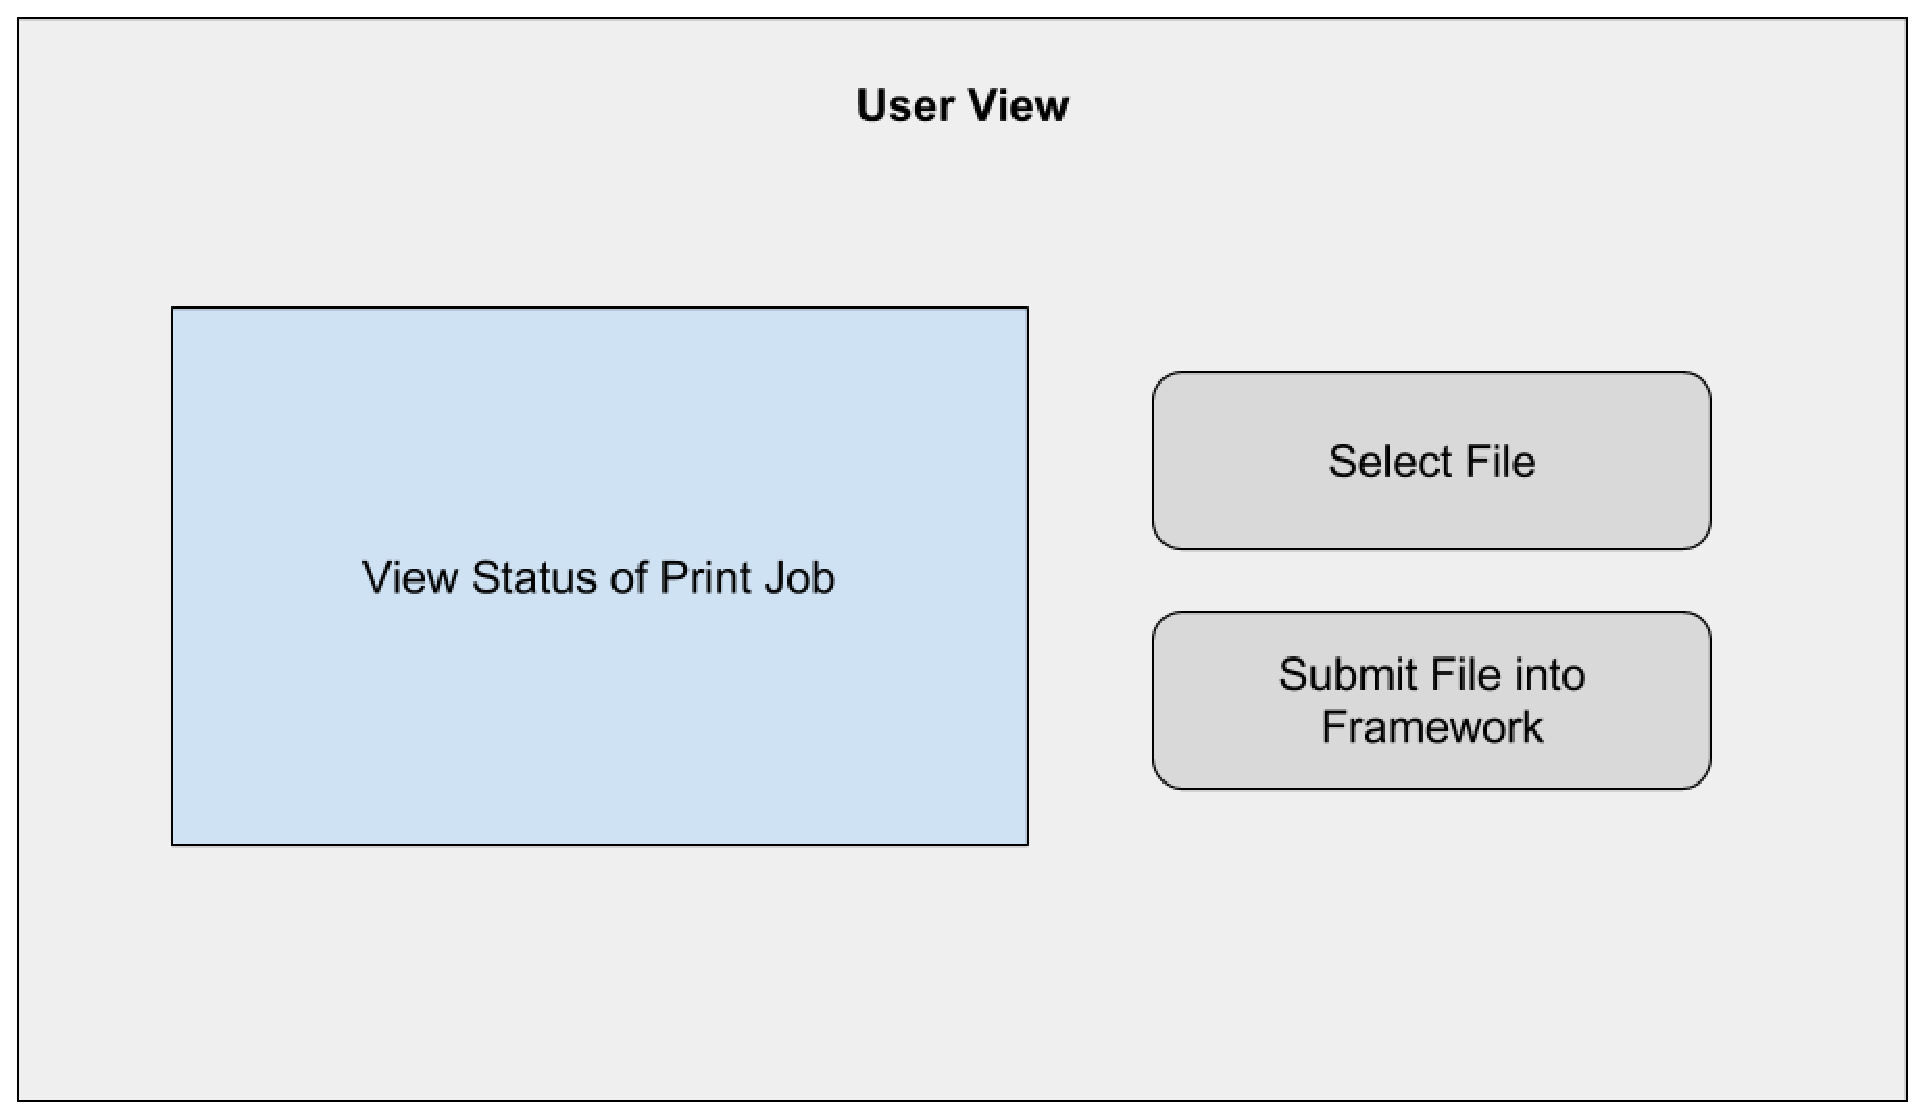
\includegraphics[scale=0.4]{user}
\captionsetup{justification=centering}
\caption{This figure shows a simple wire frame view of a user interface}
\end{figure}
% \subsubsection{Graphic}
% A graphical representation of a node in the framework will display the current system state. This graphical representation will show the latest known nodes within the system, and the services they can perform. This graphic changes dynamically as nodes enter and exit the system. When one node is in a "busy" state while accomplishing a service, it is still shown in the diagram, but is slightly grayed out. A node will no longer appear in the system when there is no signal received from them after a timeout period. 
% \subsubsection{Objective Input Button}
% Another portion of the main GUI is the objective input button. This button is for the user to pick a file to upload to the framework to be completed. Above the button is a text box with the filename of the file input. Once the file has been picked the user can choose to submit it into the system or cancel the submission.

\subsection{Observer Design}
An observer interface will include the ability for the observer to view detailed configuration and system state information. It will include the ability for these observers to see a list of all the nodes on the network, their status, and the services these nodes offer.
\begin{figure}[H]
\centering
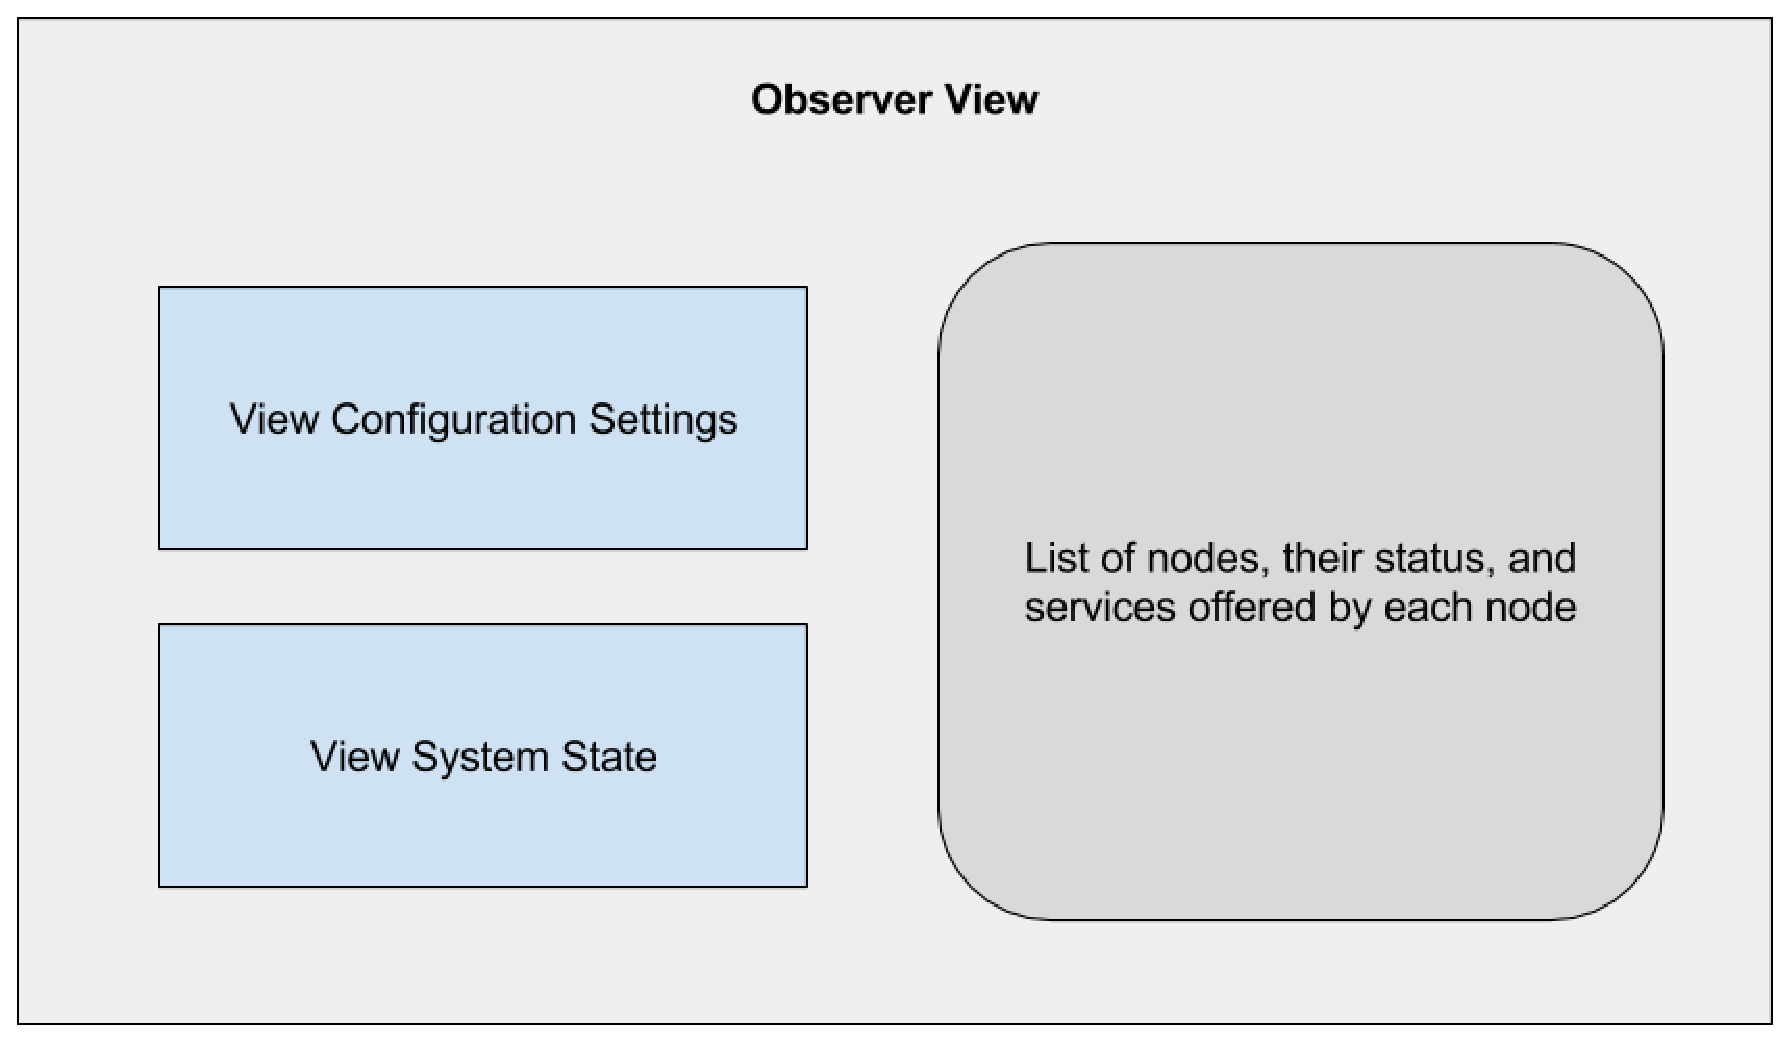
\includegraphics[scale=0.4]{observer}
\captionsetup{justification=centering}
\caption{This figure shows a simple wire frame view of an observer interface}
\end{figure}


\subsection{Administrator Design}
The administrator design is very similar to that of the observer, but the GUI contains more technical information and gives more options. Some of these different options include disabling services on different nodes by selecting the node, then selecting its respective service and clicking on a disable button. The disable button will disable currently disabled services the node is capable of doing and enable currently disabled services the node is capable of doing. 
The administrator would need to access the administrators web page by connecting to a different port of the same IP address.  
\begin{figure}[H]
\centering
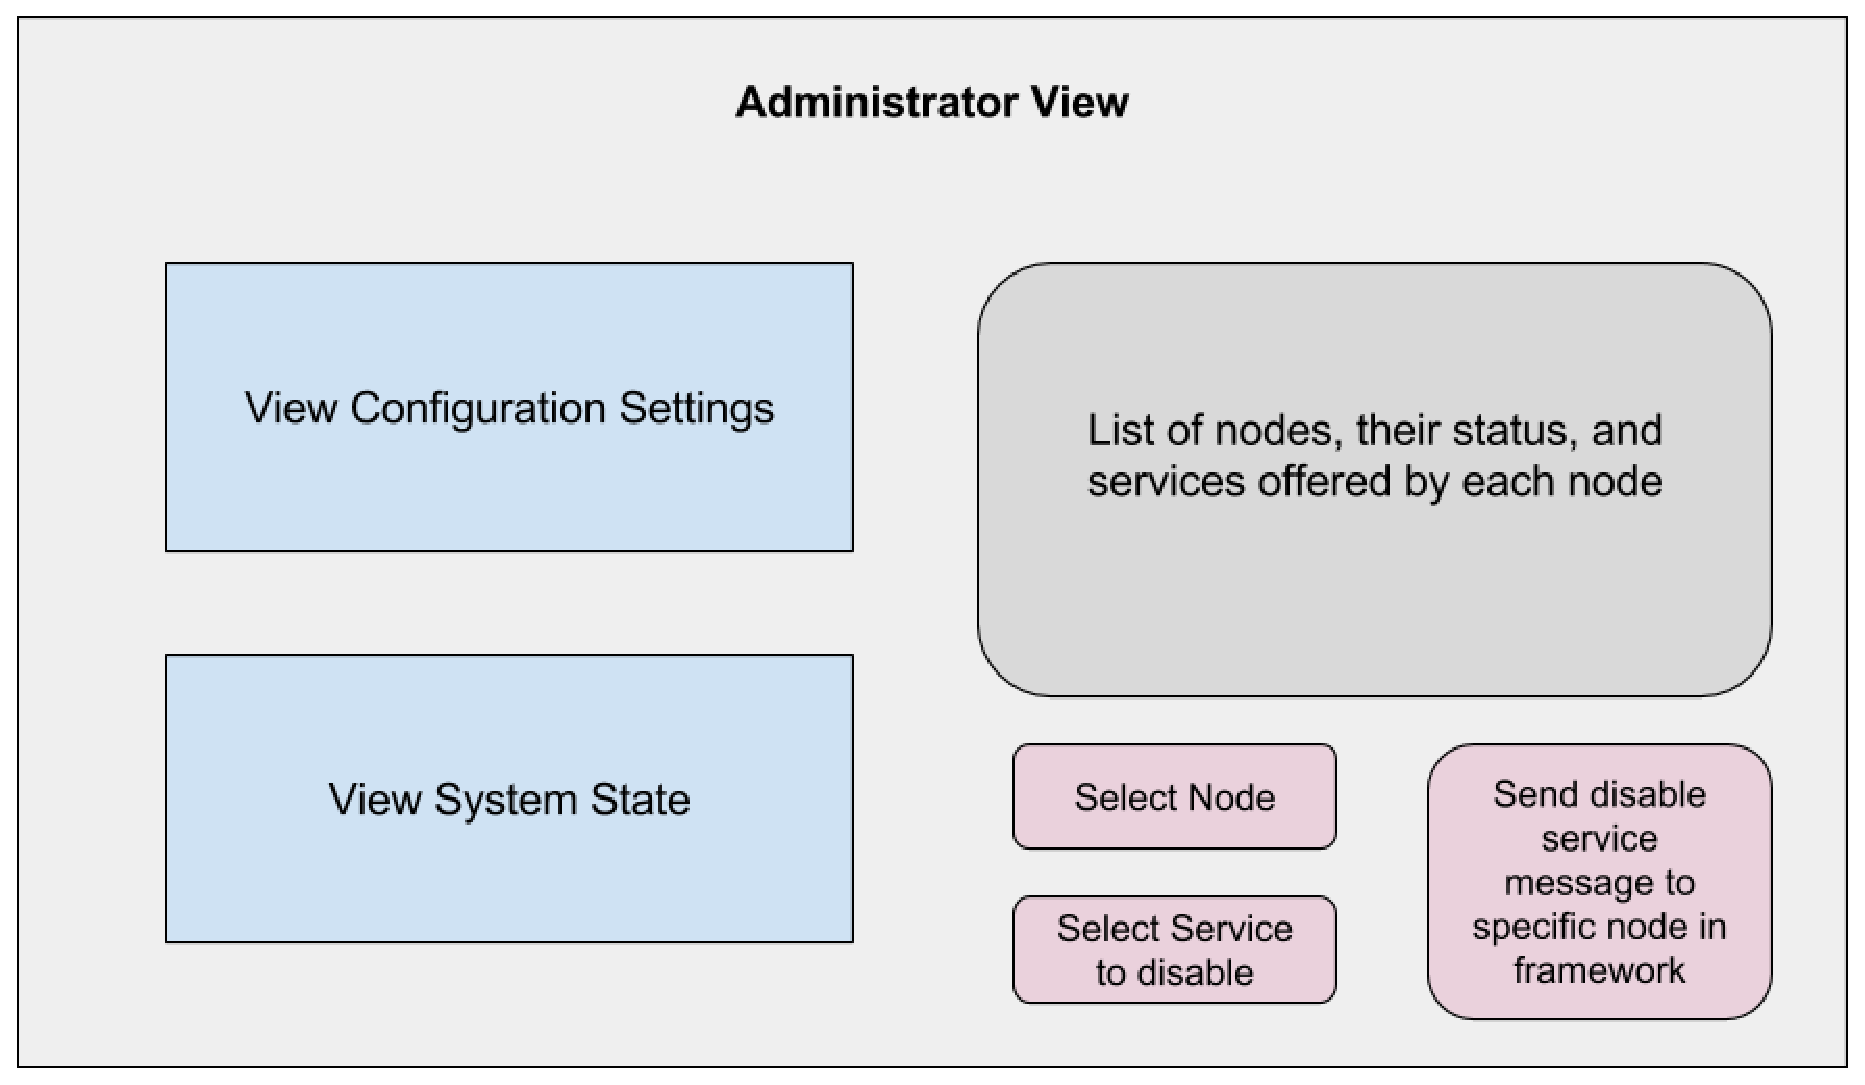
\includegraphics[scale=0.4]{admin}
\captionsetup{justification=centering}
\caption{This figure shows a simple wire frame view of the administrator interface}
\end{figure}




\section{Summary}
This framework will create a network of loosely coupled nodes that will communicate using a simple messages. It will enable users to input print job objectives into our framework and view the results from a graphical user interface. Nodes will be robust in the face of any mistrusted node. By being a robust framework, it will be able to accomplish objectives without each node having rigid logical configurations. The framework will use a combination of software and hardware. This software will contain core framework functionality, along with the graphical user interface. In the end, this framework will use a combination of software and hardware to enable a collection of wireless, loosely coupled nodes, to self organize on an objective.







\end{document}